\section{Overview of Our Approach}\label{sec:overview}
To address the problem of cumulative attacks, we want to introduce a certain
degree of diversity and non-determinism to the program execution path. This is achieved
through using a diversified scheduling structure (Section~\ref {sec:dvs}) and
multiple VMs (Section~\ref {sec:mvm}). Like any VM-based protection schemes,
\DSVMP is supposed to be use for protecting the most critical code regions but not the entire program, in order to minimize the runtime overhead.
Our current implementation targets the x86 instruction set but the methodology itself can be
applied to other architectures.


Figure~\ref{fig:Fig.overview} depicts the system architecture of \DSVMP.
Code protection of \DSVMP follows several steps described as follows.

\begin{figure}[!t]
  \centering
  % Requires \usepackage{graphicx}
  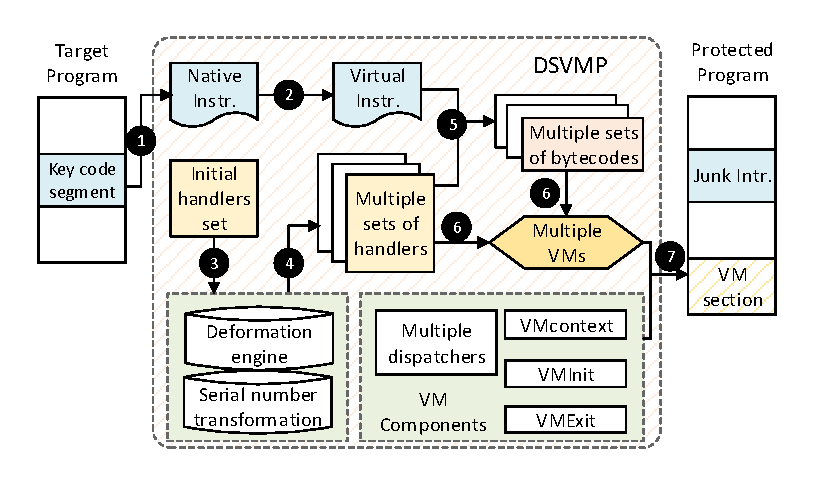
\includegraphics[width=0.7\columnwidth]{figure/figoverview.pdf}
  \caption{Offline code protection process. \DSVMP takes in a program binary. For each protected code region, it translates native instructions into bytecodes. Next, it generates multiple bytecode handlers that are semantically equivalent but implemented in different ways. It then generates the corresponding driver-data and multiple VMs. Finally, the generated VMs and associated components will be inserted into the program binary and fills the original code region with junk instructions.}\label{fig:Fig.overview}
  %\vspace{-5mm}
\end{figure}

\paragraph*{Code translation} \DSVMP takes in a compiled program binary and
does not require having access to the source code. Code segments need to be
protected are given by providing the symbolic name of the functions to be protected or the
 start and end addresses of the code blocks to be protected. The code segments are
firstly converted into native machine assembly code (e.g. x86 instructions)
using a disassembler (Step \ding{182}). The assembly code will then be mapped into a set of virtual instructions, i.e.
the intermediate language used by the VM (Step \ding{183}).
The virtual instructions will then be stored in a bytecode format.

\paragraph*{Diversifying}
As a departure from prior work on VM-based code obfuscation, \DSVMP employs multiple VM instruction scheduling policies
where each virtual instruction scheduler can have multiple dispatchers and bytecode handlers. It provides a set of handlers
that are semantically equivalent but are implemented in different ways for a single virtual instruction.
Thus, the scheduler can dynamically determine at runtime which of the handlers is used to decode a bytecode (ie. the encoding
scheme of the virtual instruction which includes the opcode and operand) and to interpret a virtual instruction.
Multiple handlers are generated by applying obfuscation to a set of seed handlers (Step \ding{184}).
The way the handlers are obfuscated could be different for different code regions.
\DSVMP also employs a multi-VM scheme by providing more than one VM implementation.
Therefore, each handler will be obfuscated for each VM by using the deformation engine (i.e. a obfuscation toolkit), resulting in $n$ (i.e. the number of VMs) sets of semantically equivalent handlers with different implementations and control flows (Step \ding{185}).
Next, the virtual instructions will be encoded into an unique bytecode form for each VM, so that the same opcode from different
VMs will be mapped into different native machine instructions to protect against static analysis.
Our preliminary implementation provides two sets of bytecode in a VM. Therefore, each
virtual instruction can be encoded into two different sets of bytecode forms in a VM(Step \ding{186}).
After these steps, \DSVMP essentially provides multiple VMs, 
where each VM contains one set of bytecode handlers (so that a virtual instruction can be interpreted by multiple handlers), 
while the instructions of the protected code regions are stored in different bytecode forms (Step \ding{187}).

\paragraph*{Code generation}
Finally, a new section will be inserted into the program binary, which contains $n$ VMs and their components such as dispatchers, \texttt{VMContext} etc. Our system also fills the original code region with junk instructions (Step \ding{188}).

This is an overview of our approach. We describe the implementation of \DSVMP in more details in the following sections.
